%!TEX root = paper.tex
%%%%%%%%%%%%%%%%%%%%%%%%%%%%%%%%%%%%%%%%%%%%%%%%%%%%%%%%%%%%%%%%%%%%%%%%%%%%%%%%
\section{Evaluation}
\label{sec:eval}

This section investigates the properties of the actual games offered on the
various platforms, so as to provide a backdrop against which utility
metrics can be viewed.
Table~\ref{tab:game-stats} provides an overview of the data.

\todo[inline]{Umsortieren um mit Background kohärent zu sein?}
\todo[inline]{Besitzzahlen für \steam anschauen?}


% %!TEX root = paper.tex

\begin{table}
\caption{Metadata for the \steam, \metacritic, \hltb, \psnow, and \gfnow datasets. Records with a * note include games from other platforms than PC, PlayStation, and GeForce Shield.}
\label{tab:dataset-metadata}
\centering
\begin{tabu}{X[1.5]|X[r]|X[0.7,r]|X}
\toprule
Product & Date generated & \# of records & Method of generation\\
\midrule
\steam & 2015-07-14 & \num{5996} & Steam \& SteamSpy\\
\steam & 2015-10-30 & \num{6769} & Steam \& SteamSpy\\
\steam & 2016-02-06 & \num{7749} & Steam \& SteamSpy\\
\psnow & 2016-02-09 & \num{190} & Official list\\
\gfnow & 2016-02-12 & \num{69} & Manual screen scraping\\
\metacritic & 2016-03-02 & * \num{46197} & Web scraping\\
\hltb & 2016-03-01 & * \num{18433} & Web scraping\\
\bottomrule
\end{tabu}
\end{table}

% %!TEX root = paper.tex

\begin{table*}
\centering
\caption{Overview of datasets. Values with * are 99th percentiles chosen due to unrealistically large outliers.}
\label{tab:dataset-stats}
\begin{tabular}{c|c|r|r|r|r|r|r}
Dataset & Metric & Mean & Min & 1Q & Median & 3Q & Max\\
\hline
\hline
\steam & Number of records & \num{7749} & -- & -- & -- & -- & -- \\
\steam & Owners & \num{218112} & \num{0} & \num{4831} & \num{21740} & \num{107299} & \num{58666968} \\
\steam & players 2weeks & \num{9064} & \num{0} & \num{0} & \num{509} & \num{1526} & \num{7860554} \\
\steam & players forever & \num{138322} & \num{0} & \num{1780} & \num{9408} & \num{51997} & \num{58666968} \\
\steam & Average playtime (forever) & \num{507} & \num{0} & \num{93} & \num{200} & \num{429} & \num{45540} \\
\steam & Median playtime (forever) & \num{246} & \num{0} & \num{36} & \num{101} & \num{216} & \num{67538} \\
\steam & average 2weeks & \num{144} & \num{0} & \num{0} & \num{48} & \num{173} & \num{11387} \\
\steam & median 2weeks & \num{126} & \num{0} & \num{0} & \num{35} & \num{128} & \num{11387} \\
\steam & Price & \num{564} & \num{-1.26} & \num{0.99} & \num{3.39} & \num{7.49} & \num{119.00} \\
\hline
\psnow & Number of records & \num{252} & -- & -- & -- & -- & -- \\
\psnow & Rental fee for 4 hours & \num{3.02} & \num{1.99} & \num{1.99} & \num{2.99} & \num{2.99} & \num{22.99} \\
\psnow & Rental fee for 7 days & \num{5.48} & \num{1.99} & \num{3.99} & \num{4.99} & \num{5.99} & \num{14.99} \\
\psnow & Rental fee for 30 days & \num{8.40} & \num{3.99} & \num{5.99} & \num{6.99} & \num{7.99} & \num{22.99} \\
\psnow & Rental fee for 90 days & \num{12.57} & \num{3.99} & \num{7.99} & \num{8.99} & \num{14.99} & \num{49.99} \\
\hline
\gfnow & Number of records & \num{68} & -- & -- & -- & -- & -- \\
\gfnow & Price & \num{6.98} & \num{0} & \num{0} & \num{0} & \num{13.99} & \num{59.99} \\
\hline
\metacritic & Number of records & \num{45803} & -- & -- & -- & -- & -- \\
\metacritic & User score & \num{6.9} & \num{0} & \num{6.2} & \num{7.3} & \num{8.1} & \num{9.3} \\
\metacritic & Score & \num{69} & \num{8} & \num{62} & \num{72} & \num{79} & \num{96} \\
\hline
\hltb & Number of records & \num{18129} & -- & -- & -- & -- & -- \\
\hltb & Main story length & \num{26} & \num{0.02} & \num{2.5} & \num{6} & \num{12} & * \num{94} \\
\hltb & Main extra length & \num{21} & \num{0.08} & \num{5} & \num{10} & \num{20} & * \num{126} \\
\hltb & Completionist length & \num{28} & \num{0.03} & \num{5} & \num{13} & \num{29} & * \num{250} \\
\hltb & Combined length & \num{13} & \num{0.02} & \num{3} & \num{8} & \num{15} & \num{420} \\
\end{tabular}
\end{table*}

\todo[inline]{PZ: Viele daten, aber welche plattform ist die beste?}


%%%%%%%%%%%%

\begin{table*}
\centering
\caption{Game characteristics on the investigated platforms. Title counts from Web/API scraping, lengths from \hltb, ages and review scores from \metacritic.}
\label{tab:game-stats}
	\begin{tabu}{X[2]|X[r]X[r]X[r]X[r]X[r]X[r]X[r]}
	\toprule
	Service & Titles & Age $\mu$ & Age $\sigma$ & Length $\mu$ & Length $\sigma$ & Score $\mu$ & Score $\sigma$ \\
	\midrule
	\gfnow & $68$ & \SI{2.87}{\year} & \SI{1.95}{\year} & \SI{14.65}{\hour} & \SI{14.44}{\hour} & $75.9$ & $9.44$ \\
	\psnow & $191$ & \SI{5.24}{\year} & \SI{2.55}{\year} & \SI{12.26}{\hour} & \SI{15.47}{\hour} & $76.72$ & $11.43$ \\
	\steam & $7749$ & \SI{3.36}{\year} & \SI{3.95}{\year} & \SI{13.02}{\hour} & \SI{20.49}{\hour} & $71$ & $12$ \\
	\bottomrule
	\end{tabu}
\end{table*}


%%%%%%%%%%%%
\subsubsection{Number of Games}

The two cloud
platforms offer a very limited number of games when compared to the
games available on \steam, which itself again only represents a subset
of all games available either on the PC platform (\metacritic lists
$16192$) or across all platforms ($45803$ listed on the site). Two
possible, simple explanations for the low game count on the cloud
platforms come to mind: One is that they were launched relatively
recently (2015) in comparison to \steam (2003), leaving little time for
the range of games to grow. Secondly, the choice of games for a cloud
gaming platform is most likely curated by the platform operator for
compatibility and performance reasons. This usability burden shifts to
the end user for digital storefronts like \steam, allowing these
platforms to offer a larger variety of games, including ones that are
very demanding on the hardware.


%%%%%%%%%%%%
\subsubsection{Game Ages}

Game ages appear to be relatively high for all of the investigated
platforms, and particularly so for \psnow. It might be considered a
special case, as it is specifically advertised as a backwards
compatibility for older, pre-PlayStation 4 games that do not run on the
latest Sony platform any more. For \steam, the distribution is
significantly skewed towards recent titles: A quarter of games are less
than $10$ months old, and the median is at $21$ months. The
distribution's tail extends well beyond $25$ years (due to re-releases
of ``classic'' games on the platform).


%%%%%%%%%%%%
\subsubsection{Game Lengths}
Figure~\ref{fig:gamelengths-violin} shows the distribution of aggregated
game lengths for the three platforms under investigation, and an
``overall'' distribution that includes further platforms and gaming
systems. Among the three platforms, the mean and median reported game
lengths (approximately \SI{14}{\hour}) are largest for \gfnow. In
contrast to the curated choice of games on the Cloud systems, \steam
also offers shorter and longer games.


\begin{figure}[!t]
	\centering
	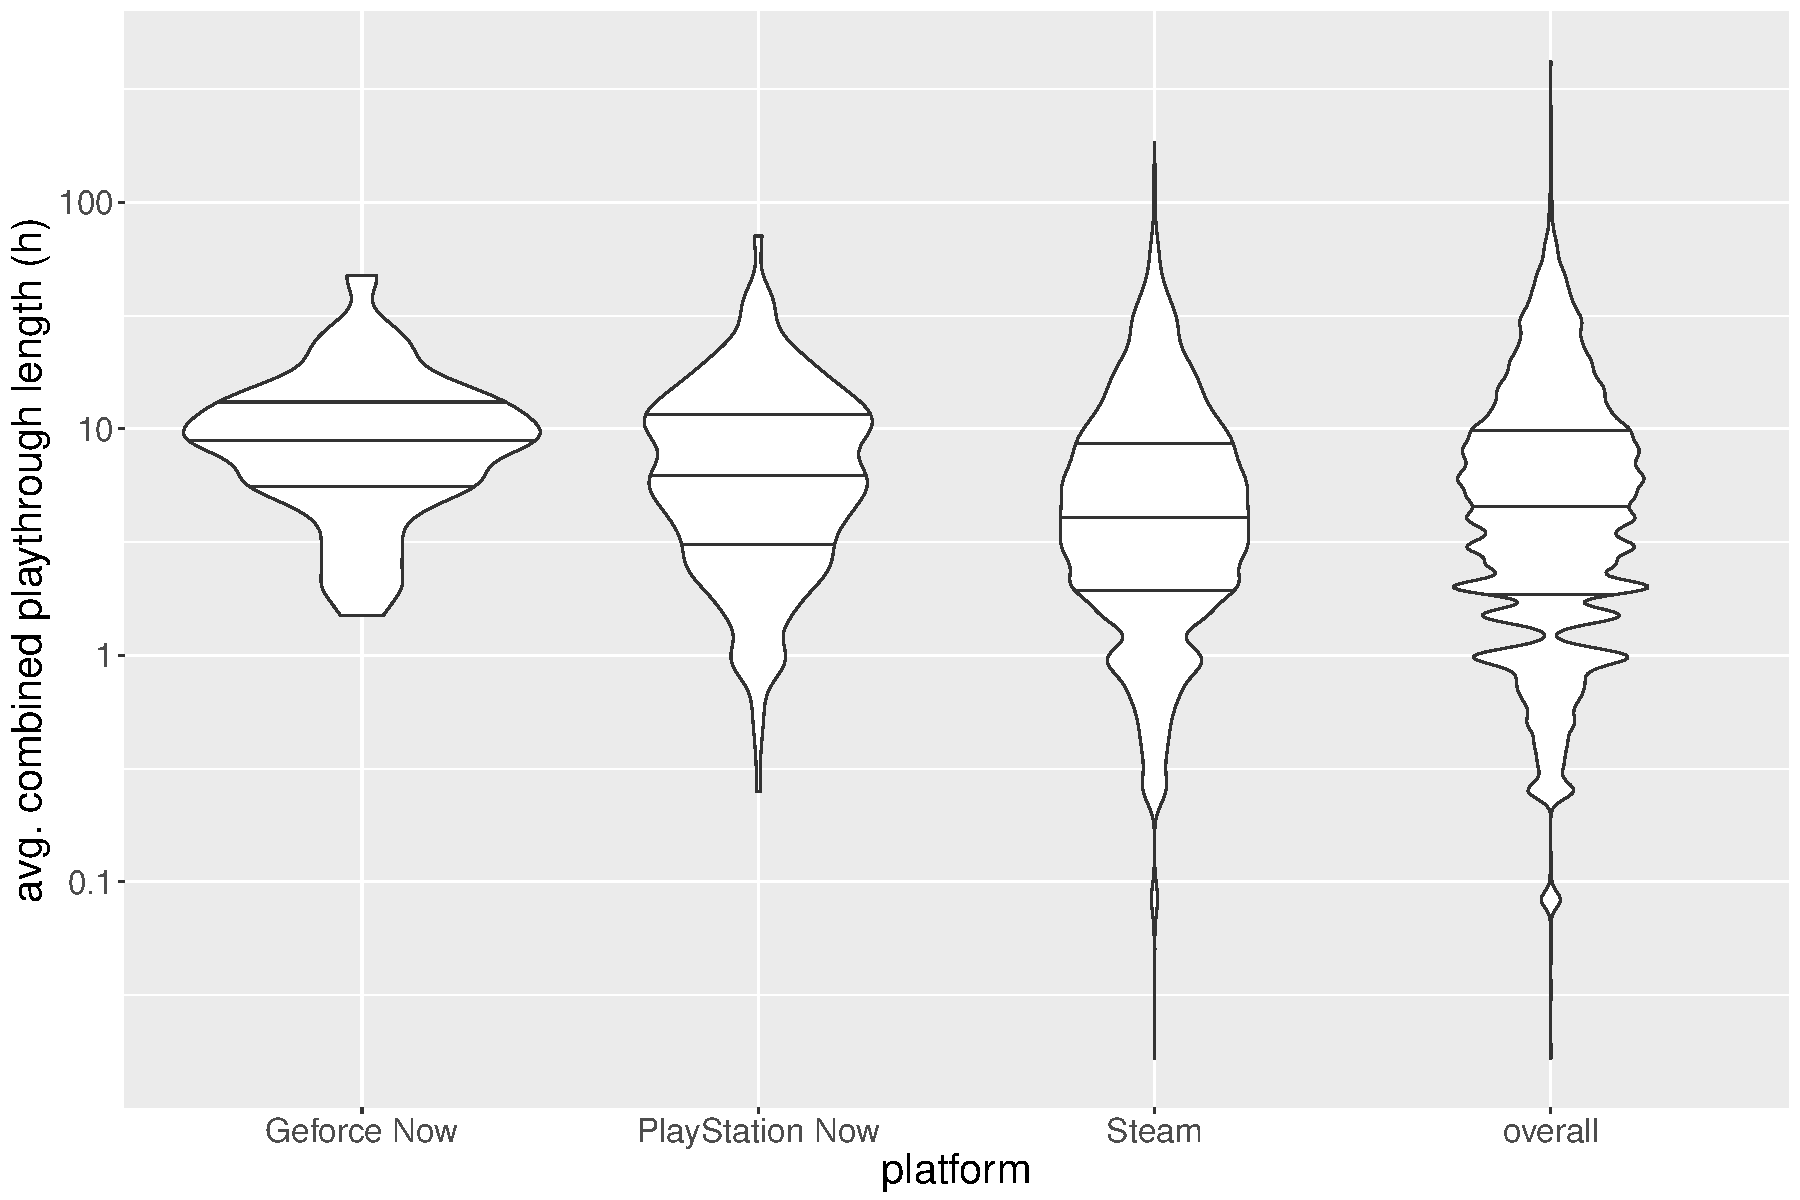
\includegraphics[width=1.0\columnwidth]{images/gamelengths-by-platform-violin.pdf}
	\caption{Violin plot of the per-platform average game lengths from \hltb. The number of games per bin are $68$, $209$, $7764$, and $18433$; quartiles indicated by horizontal lines.}
%	aggregated over all play styles (raw data source: \hltb).}
\label{fig:gamelengths-violin}
\end{figure}



%%%%%%%%%%%%
\subsubsection{Game Prices}

Trying to compare the prices per game is a difficult endeavor, due to
the mixed approach of both cloud gaming platforms. The \gfnow
subscription gives you access to a subset of its catalog that can be
extended by purchasing additional games. Similarly, \psnow has a base
subscription catalog and additional, rentable titles. But in addition,
every title can also be rented without the need for an active
subscription.
%; at the same time, further titles may be bought in addition (on \gfnow), or an alternative, à la carte purchase option besides subscription exists (on \psnow). 
%\todo[inline]{SV: So, both platforms have a mixed approach? You rent the games, but can parallely buy them? I didn't understand the second sentence and just erased it (/commented it out).}
%Furthermore, the exact subscription and rental modalities as well as prices are adapted over time, and differ between regional markets.
%\todo[inline]{SV:The last sentence was somehow superfluous since variety over time is the case for all of our data. --> erased it.}
For \steam on the other hand, unit prices can be discussed.

\begin{table}
\centering
\caption{Overview of average prices and counts for \steam games.}
\label{tab:steam-price-stats}
\begin{tabu}{X[2]|X[r]X[r]X[r]X[r]X[r]X[r]X[r]X[r]}
	\toprule
	\textbf{Date} & 2015-07 & 2015-10 & 2016-02 & 2016-06 & 2016-09 & 2016-11 & 2017-04 & 2017-10 \\
	\midrule
	\textbf{Average price (€)} & $10.11$ & $8.47$ & $5.65$ & $4.72$ & $8.77$ & $5.33$ & $9.95$ & $8.83$ \\
	\midrule
	\textbf{Standard deviation (€)} & $\pm12.03$ & $\pm9.74$ & $\pm7.88$ & $\pm7.02$ & $\pm10.83$ & $\pm11.08$ & $\pm29.94$ & $\pm12.2$ \\
	\midrule
	\textbf{Number of games} & $5,996$ & $6,769$ & $7,749$ & $9,187$ & $10,191$ & $10,077$ & $11,612$ & $14,120$ \\
	\bottomrule
\end{tabu}
\end{table}

Table~\ref{tab:steam-price-stats} shows the development of average
\steam game prices with standard deviations and the number of available
games for all \steam measurements taken so far.
\todo[inline]{Update this!}
 Two different types
of averages are shown: The portfolio price which averages over all
current game prices, and the weighted price which is the product of game
price and estimated number of owners, averaged over the total number of
games owned. Strong temporal effects are evident from either metric.
Note that the last measurement shortly predates 2016's Lunar New Year,
around which \steam ran a large seasonal sales
campaign\footnote{\url{http://store.steampowered.com/news/20313/}}.

% Looking at the distributions of game prices, we find that the number of games in the sub \SI{5}]\EUR] category has ... hmm, what ... doubled? ... care to check with R?

%The influence of sales periods can be easily observed in the \acrshort{CDF} of prices in Fig. \ref{fig:steam-prices}, where the data from February was collected during \steam's Lunar New Year Sale.

%\begin{figure}[!t]
%	\centering
%	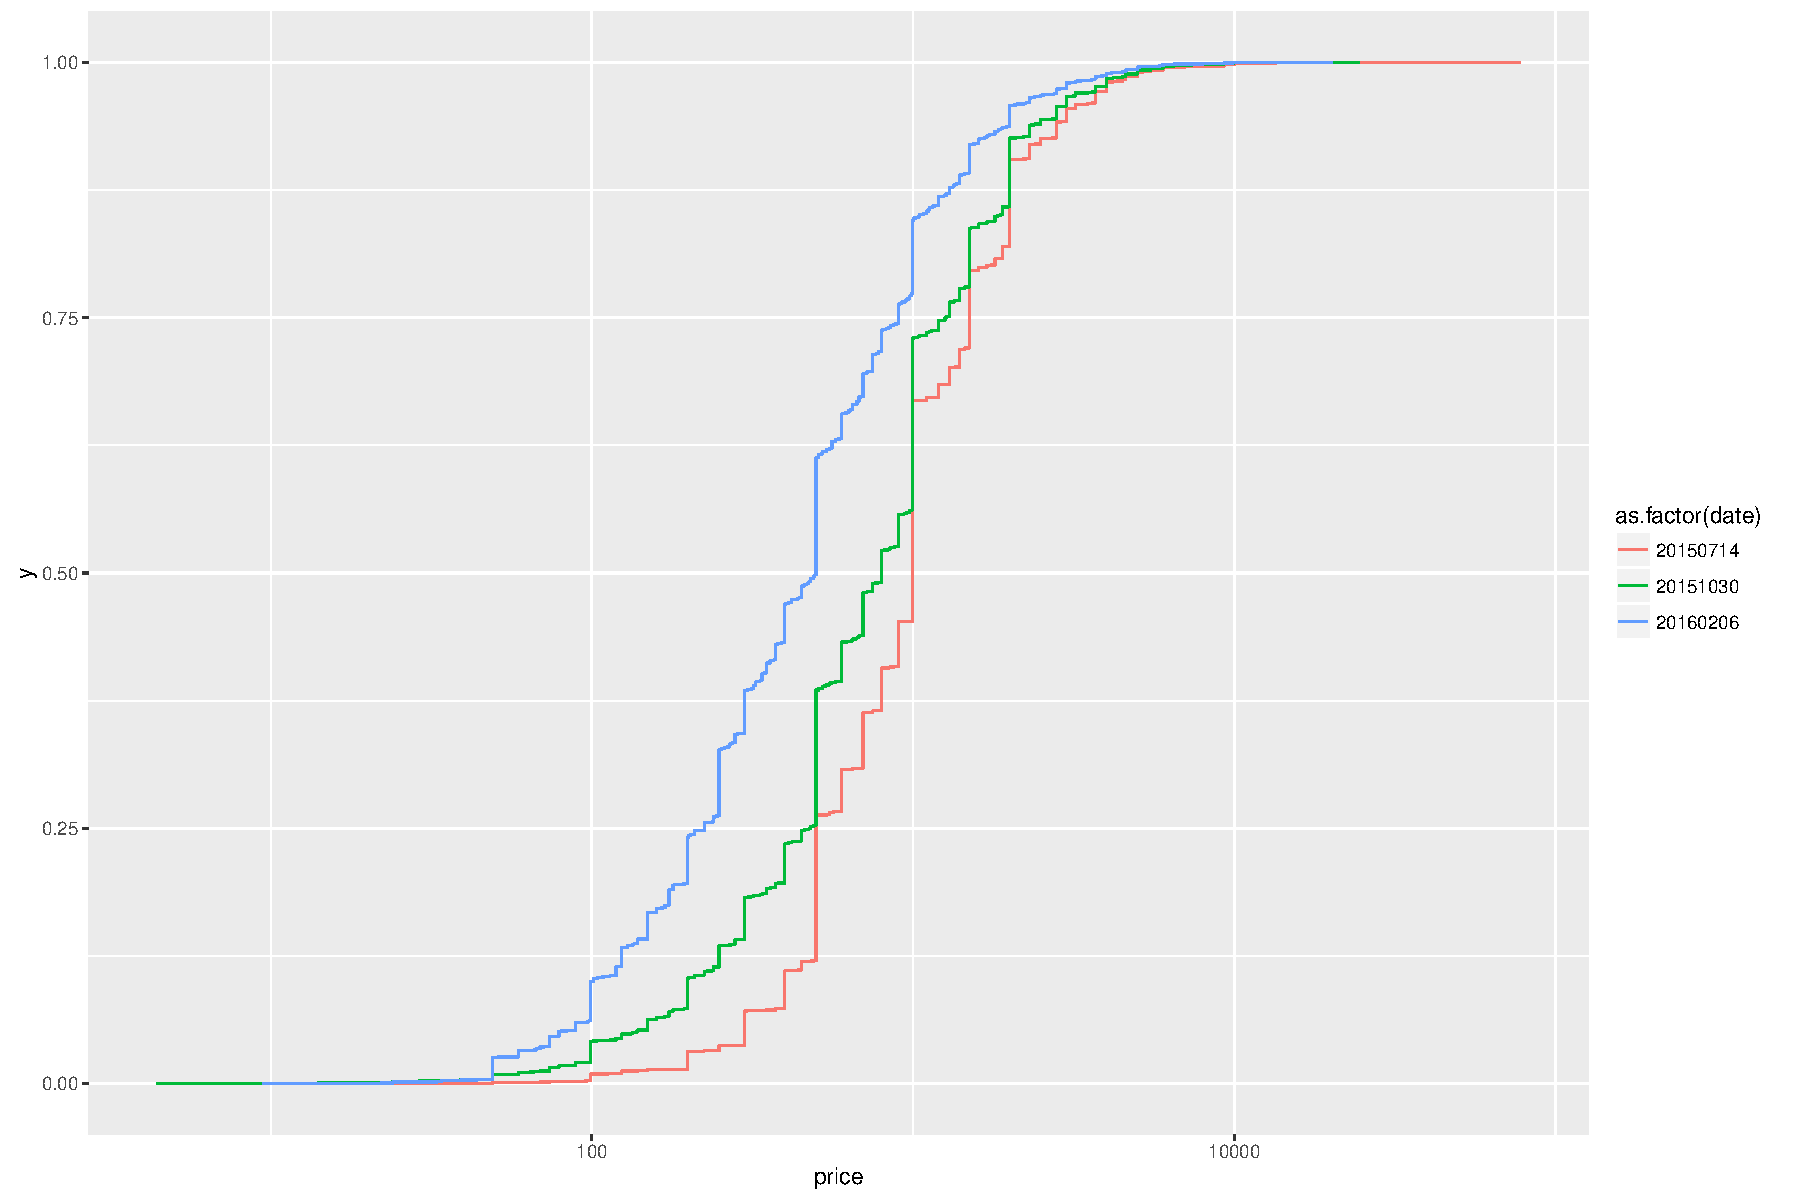
\includegraphics[width=1.0\columnwidth]{images/steam-prices.pdf}
%	\caption{CDF of games on the \steam platform at three distinct dates. The February data was collected in a sales period.}
%\label{fig:steam-prices}
%\end{figure}

\begin{figure}[!t]
	\centering
	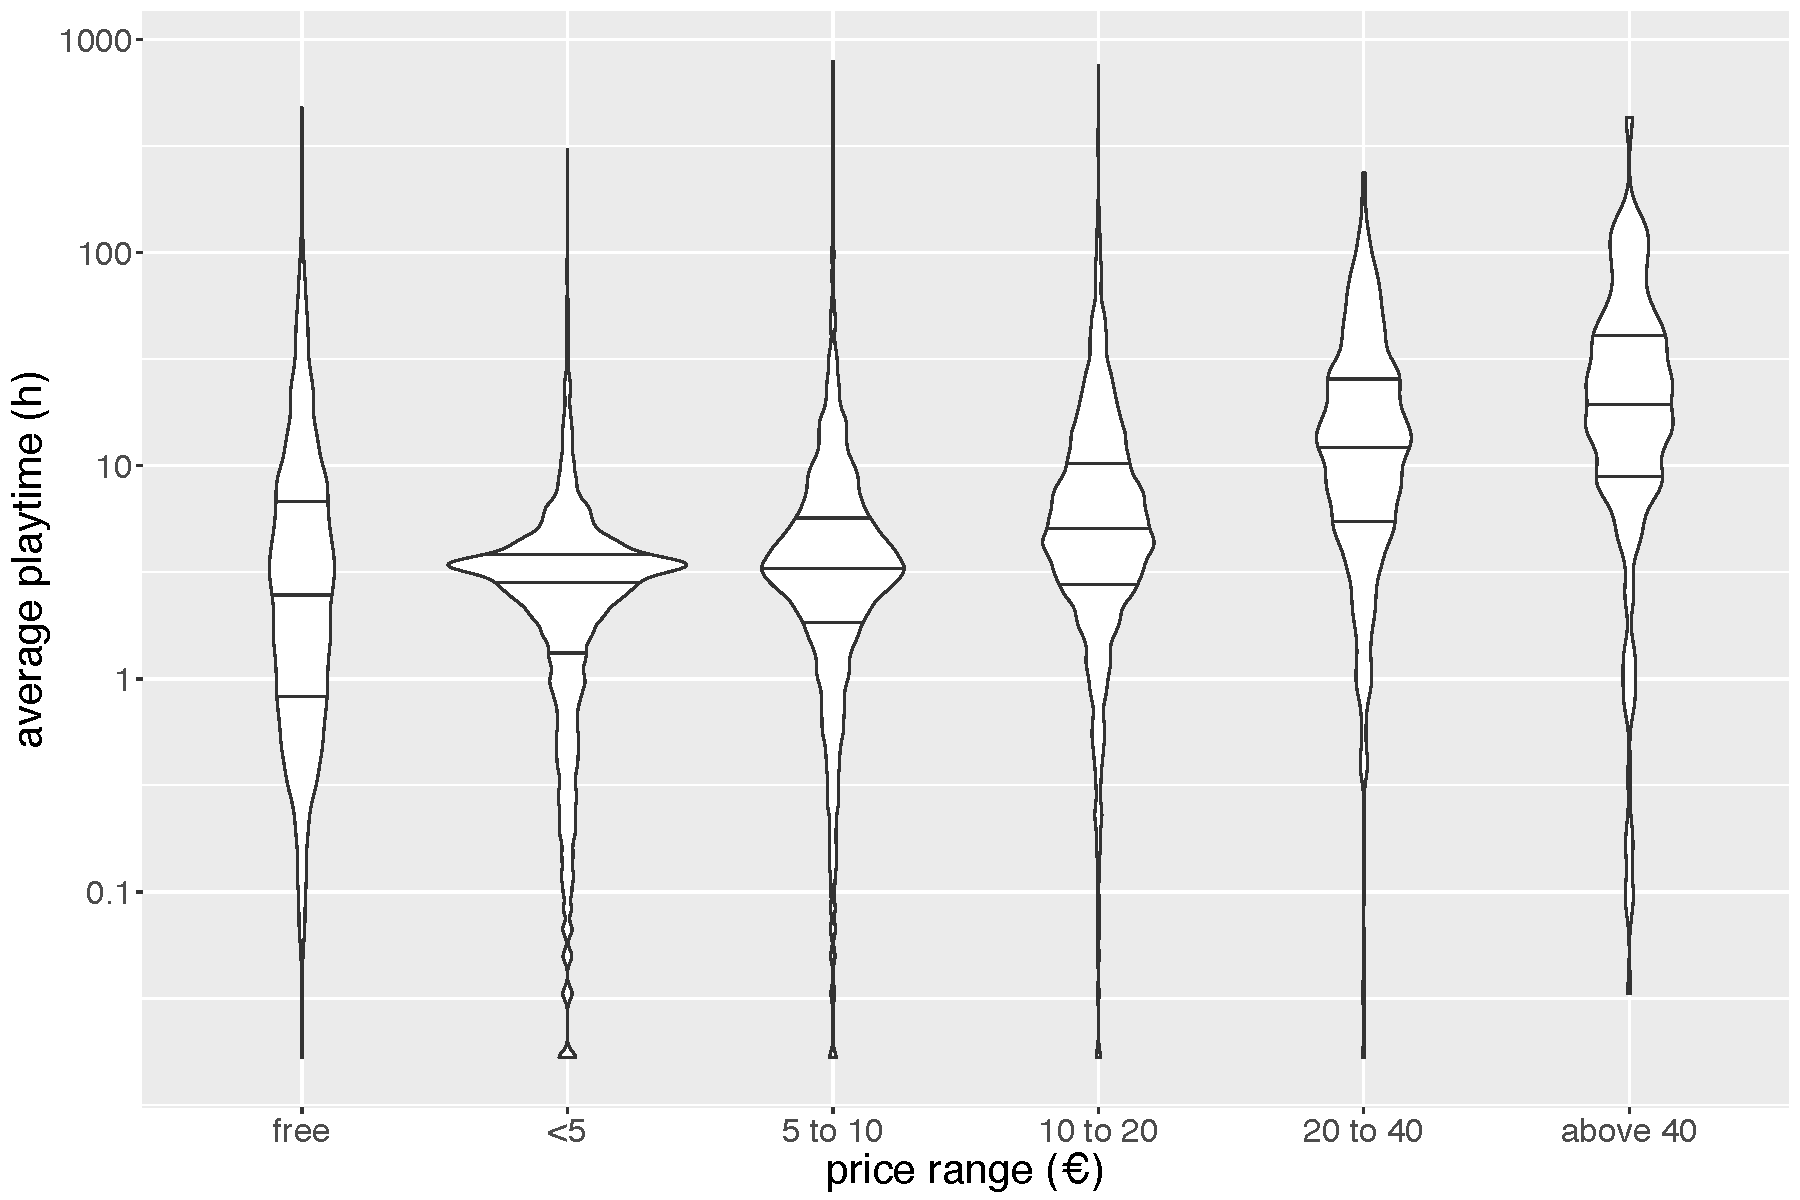
\includegraphics[width=1.0\columnwidth]{images/steam-cost-vs-playtime-non-sale.pdf}
	\caption{Violin plot of the average playtime of \steam games, broadly categorized by their prices. The number of games per bin are $1541$, $5269$, $4019$, $2445$, $658$, and $188$.}
\label{fig:steam-cost-vs-playtime-violin}
\end{figure}

\subsubsection{Price versus Playtime}
Again focusing on \steam,
Figure~\ref{fig:steam-cost-vs-playtime-violin} breaks down the
distribution of average playtimes per game price range. The game price
ranges are chosen so as to roughly separate the prevalent modes of the
price distribution.
% AR: The modes would be approximately 1, 2, 5, 10, 15, and 20 Euros from visual inspection of images/steam-prices-density.pdf.
Playtime is defined as the time game owners spend playing a game, as
recorded by the \steam platform and scraped from \textit{SteamSpy}. As
can be seen, the playtimes generally increase with the price range;
unfortunately, the data does not explain the cause: E.g., more expensive
games might have more playable content, causing the playtime to
increase. Conversely, higher upfront costs may incite players to spend
more time regardless of game quality, thus avoiding regret for the
expense. On the far left in the Figure, playtimes of ``free'' titles
(including free-to-play games with monetization options other than an
upfront payment) span almost the whole playtime range with less
pronounced prevalences.
% Svenja deleted the following sentence since that can be the case anywhere:
%And still alternatively, there might exist an outside, common reason causing both parameters to increases.
Due to the strong popularity of \steam in PC gaming (even physical
retail copies often require using the service nowadays) this set also
gives a good overview of the dimensions of PC gaming in general.


%%%%%%%%%%%%
\subsubsection{Review Scores}

The final characteristic in this analysis are game review scores as
given by professional gaming media outlets. This relies on the
\metacritic dataset again. This set covers review scores for all current
and historic gaming platforms. The review scores are aggregated to
average scores ranging between $0$ and $100$. Some \metacritic-internal
weighing factors are applied to express the importance of some media
outlets over others.
The average scores seem quite similar across all services, albeit with a
slightly lower $\sigma$ for \gfnow. Figure~\ref{fig:scores-by-platform}
shows the distribution of review scores per platform. Both Cloud
services seem to favor certain score levels. Specifically, their lowest
quartiles (representing the worst-rated games on these platforms) reach
much higher values than \steam's. This could be an effect of the Cloud
systems curating the game offer to focus on highly-rated (and thus
perhaps more attractive) titles. \steam on the other side is a more or
less open platform, where every game publisher can sell their games at
their own volition (platform operator collects a commission fee for
sales). Consequently, it is reasonable to assume more variation in the
quality of games, which could in turn lead to mixed reviews.
%Cloud gaming platforms have to acquire licenses from the individual games' publishers and therefore have to be selective and curated by nature.
%\todo[inline]{AR: Should we mention other possible effects such as ``Metacritic probably isn't free of bias (gosh!)''?}
% that would only lead to a very, very lengthy off-topic discussion, so probably no

% TODO: include or compare with data from opencritic.com as soon as their API is public/usable

% \begin{figure}[!t]
% 	\centering
% 	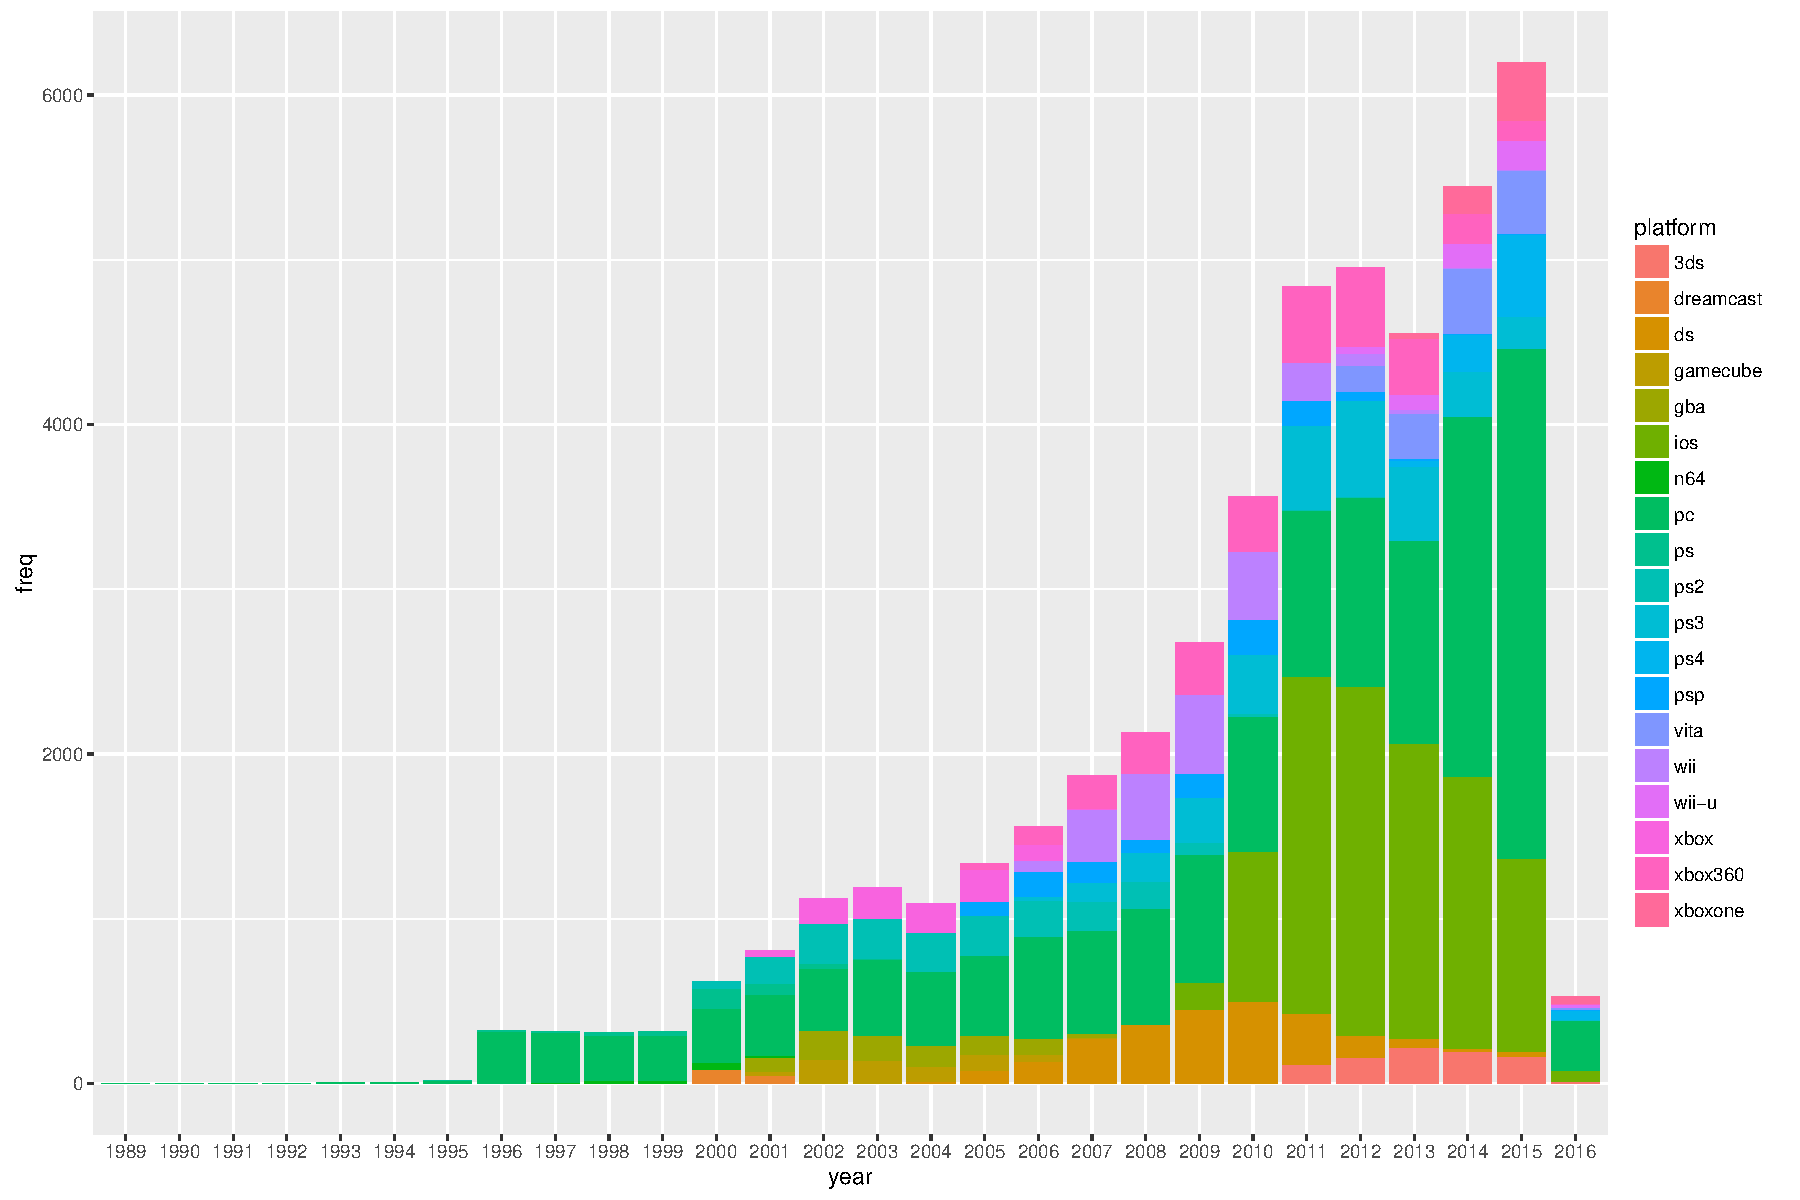
\includegraphics[width=1.0\columnwidth]{images/releases-per-year.pdf}
% 	\caption{Number of game releases per platform according to the Metacritic data.}
% \label{fig:releases-per-year}
% \end{figure}

\begin{figure}[!t]
	\centering
	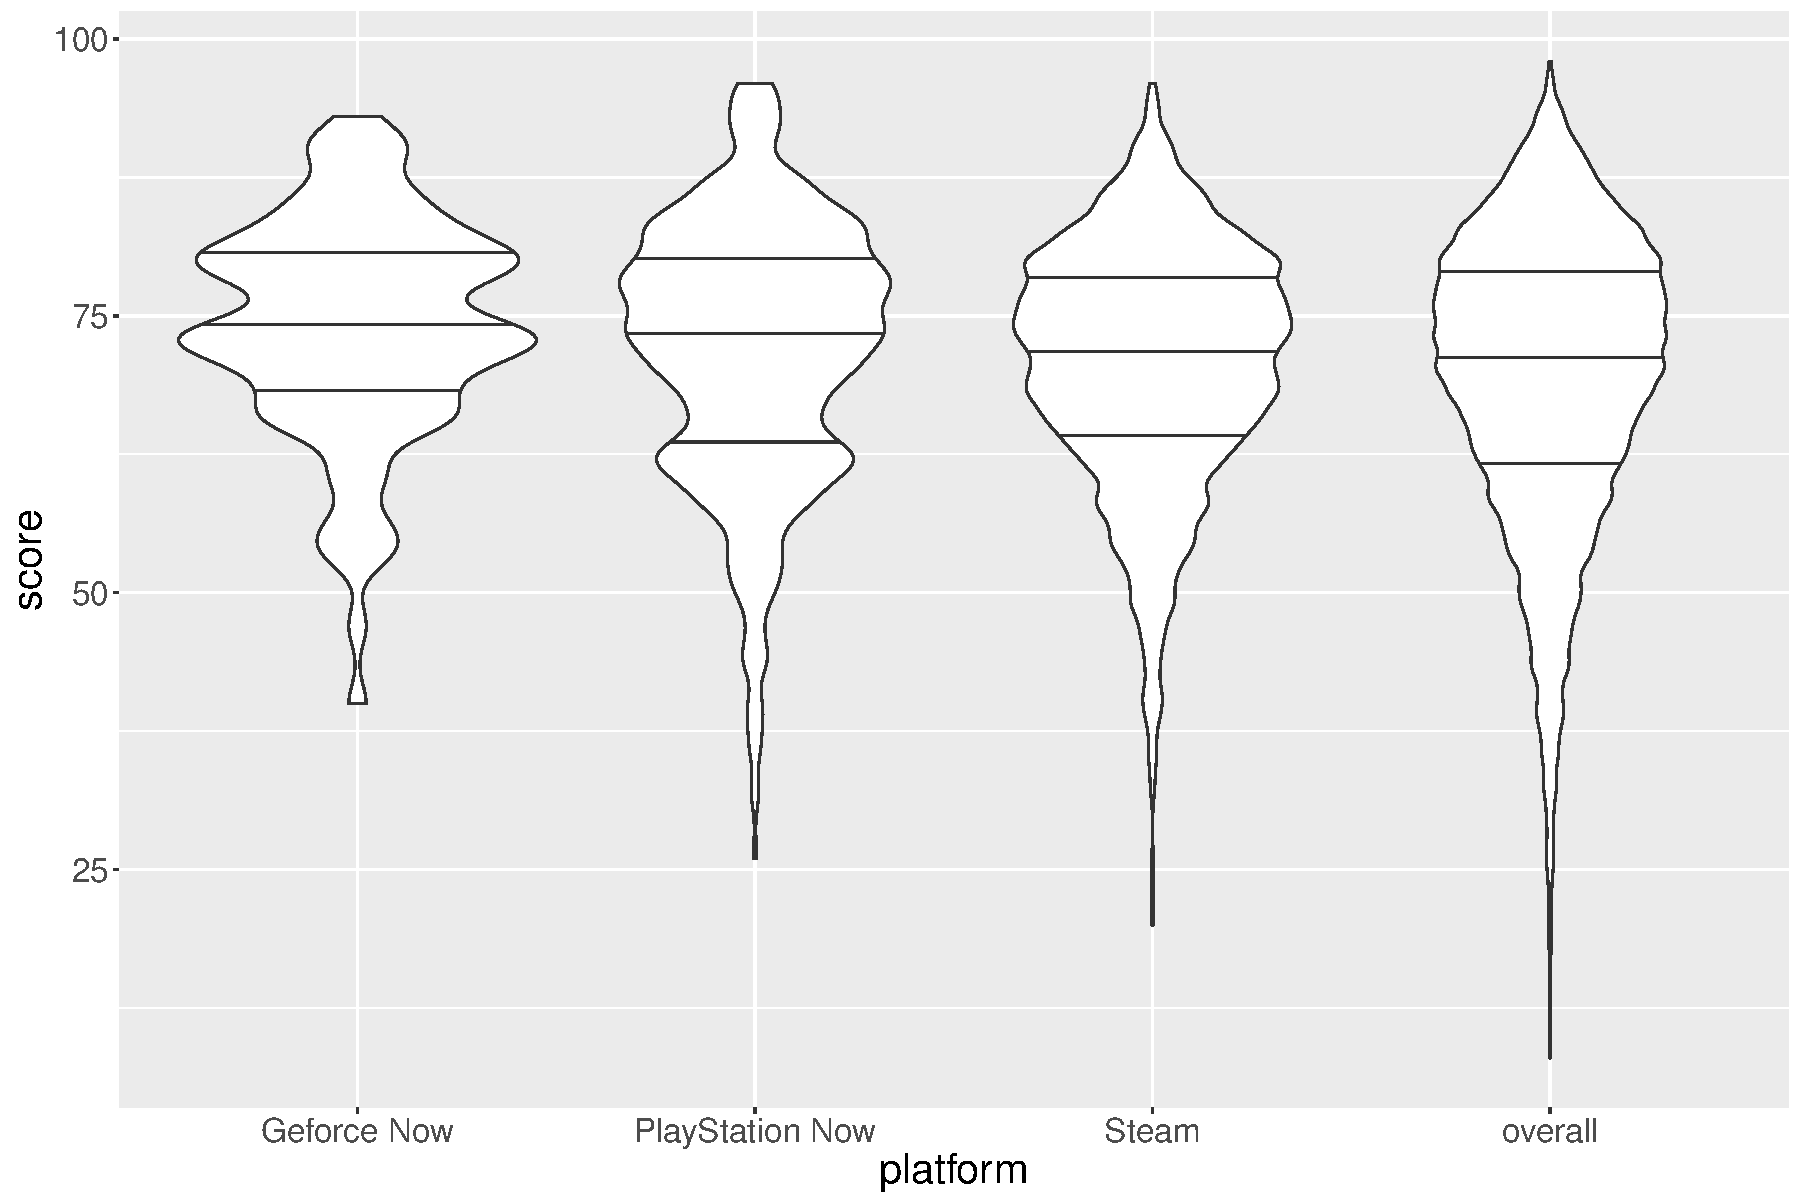
\includegraphics[width=1.0\columnwidth]{images/scores-by-platform-violin.pdf}
	\caption{Violin plot of aggregated review scores per platform. The number of games per bin are $68$, $209$, $7759$, and $46197$.}
\label{fig:scores-by-platform}
\end{figure}

